\chapter{Quantum Decoherence}
%
%\ohead{\rightmark}
%
%\ohead{\ref{subsec:decoh} New Physics Searches}
%
As it will be further explained in \cref{subsec:oqsf}, there are many phenomenological models in which quantum decoherence can manifest itself in neutrino oscillations.

\section{Phase-Perturbed Neutrinos}
An illustrative picture is given by quantum-gravity motivated scenarios in which the neutrino propagates through a quantum-fluctuating spacetime (also called spacetime foam) and experiences stochastic perturbations in the form of an interaction with a \acrfull{vbh} state. Such \acrshort{vbh}s are the gravitational analogue to virtual electron-positron pairs in the context of vacuum polarisations in quantum electrodynamics \cite{QD_Stutt_Jens_2020}. The propagation of a neutrino mass state $\ket{\nu_j}$ by some distance $L$ is given by
%
\begin{align} \label{eq:nu_mass_propagation}
    \ket{\nu_j(L)} = \hat{U}(E_k, t) \ \ket{\nu_j (0)}
    \quad \text{,} 
\end{align}
%
where the time evolution operator is given by $\hat{U}(E_j, t) = e^{-i E_j t}$. In a $2\nu$-flavour paradigm, one can evaluate $E_k t = \frac{m_k^2 L}{2E}$, which results in the standard $2\nu$-flavour transition probability. Phase perturbations resulting from quantum decoherence effects described above then introduce a shift in phase $\delta \Phi_j$, which ultimately gives rise to the damping of the neutrino oscillation probability \cite{QD_Stutt_Jens_2020}:
%
\begin{align} \label{eq:nu_mass_propagation_perturbed}
    \ket{\nu_k(L)} = e^{-i \frac{m_j^2 L}{2E} + \delta \phi_j t} \ket{\nu_j (0)}
\end{align}
%
%
In quantum mechanics, the probability of the transition from one quantum mechanical state $\psi_i$ to another state $\psi_j$ is given by the amplitude squared $\left|\braket{\psi_j|\psi_i}\right|^2$. The neutrino flavour oscillation probability (analogously for anti-neutrinos) is hence given by
%
\begin{align} \label{eq:nu_flavour_osc_prob}
    P_{\nu_\alpha\rightarrow \nu_\beta}(L) = \left|\braket{\nu_\alpha|\nu_\beta}\right|^2 = \sum_{k,j} U^{*}_{\alpha k}U_{\beta k}U_{\alpha j}U^{*}_{\beta j} e^{-i\frac{\Delta m^2_{kj} L}{2E}}
\end{align}
%
In \cref{fig:qd_demo}, the effect of the neutrino experiencing decoherence due to a $\nu$-\acrshort{vbh} interaction on the oscillation probability (caluclated using \cref{eq:nu_flavour_osc_prob} in a $2\nu$-flavour paradigm) is shown.
%
    \begin{figure}[H]
	\centering
	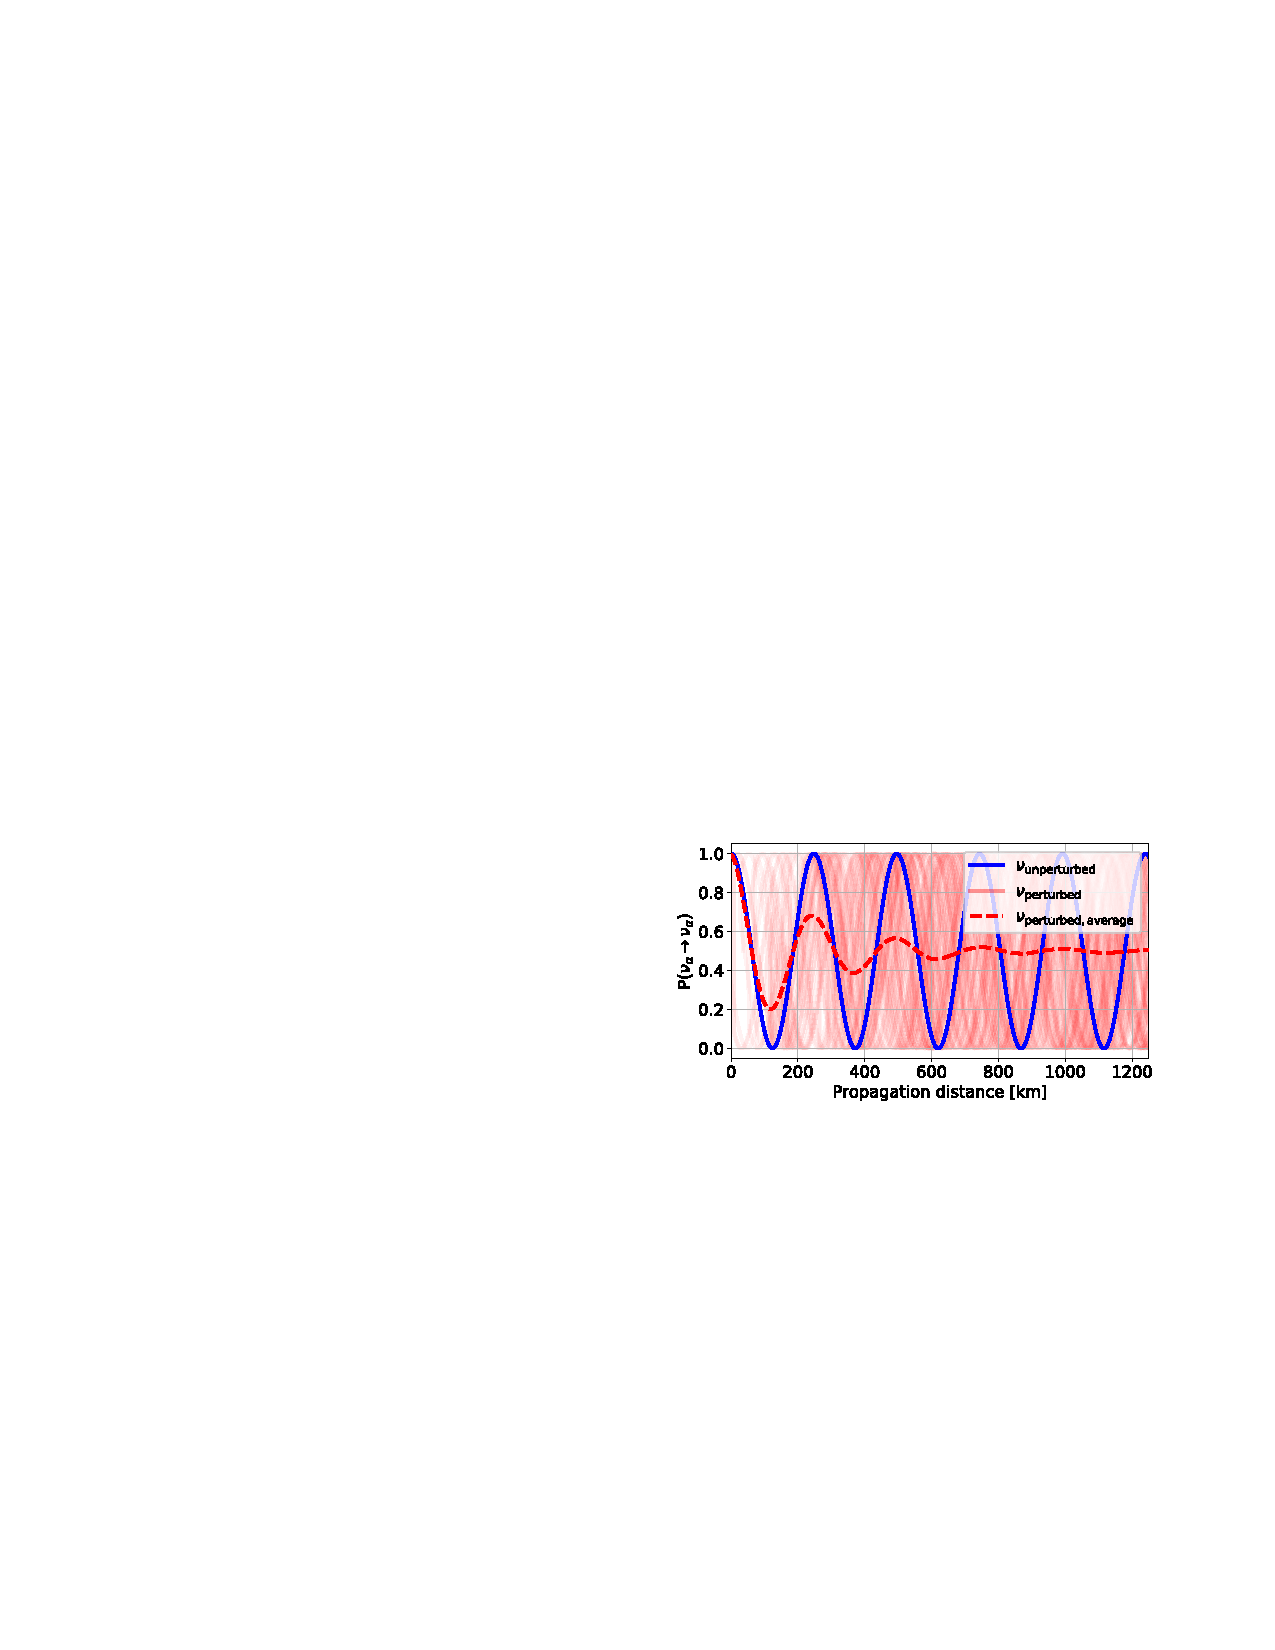
\includegraphics[width=0.85\textwidth]{figures/qd_demo.pdf}
	\caption{Demonstration of the damping of the neutrino oscillation probability due to quantum decoherence in the $2\nu$-flavour paradigm. The sum of all phase-perturbed neutrinos (one blurry red line for one neutrino) gives rise to a damped neutrino-oscillation probability (solid red line). The probability in the unperturbed case is shown in solid blue. Figure taken from \cite{QD_Stutt_Jens_2020}.}
	\label{fig:qd_demo}
    \end{figure}
%
As one can see, the stochastic perturbations of individual neutrinos result in a damping of the oscillation probability when considering the ensemble of multiple phase-perturbed neutrinos.
%\vspace{-4mm}
\section{Open Quantum Systems Formalism}\label{subsec:oqsf} 
%
%\ohead{\ref{subsec:oqsf} Open Quantum Systems Formalism}
%\label{sec:openqs} \vspace{-2mm}\label{nuclear_effects}
In the following, quantum decoherence is described in the open quantum systems formalism. Let the density matrix $\rho$ describe a system of $j$ states with a probability $p_j$ of the system being in a state $j$ according to
\vspace{-3mm}%
%
\begin{align} \label{density-matrix}
    \rho = \sum_j p_j \ket{\psi_j}\bra{\psi_j} \ .
\end{align}
%
The transition probability from neutrino flavour $\alpha$ to $\beta$ is then given by
\vspace{-3mm}%
\begin{align} \label{eq:open_sys_osc_prob}
    P_{\nu_\alpha\rightarrow \nu_\beta}(L) = Tr[\hat{\rho}_\alpha(t)\hat{\rho}_\beta(0)] \ .
\end{align}
%
In order to find $\rho(t)$ in \cref{eq:open_sys_osc_prob}, the time evolution of that system subject to the system experiencing a new physics effect is given by the Lindblad master equation \cite{Lindblad:1975ef}:
\vspace{-3mm}%
\begin{align} \label{lindblad-master-eq}
    \dot{\rho} = -i[H,\rho] - \mathcal{D}[\rho] \ \text{,}
\end{align}
%
which is an extension of the Liouville–von Neumann equation $\dot{\rho} = -i[H,\rho]$ that describes the time evolution of a density matrix in quantum mechanics. In \cref{lindblad-master-eq}, the new physics lives in the decoherence operator $\mathcal{D}[\rho]$.
The decoherence operator is expressed as a linear combination\footnote{Note that the same result for $\mathcal{D}[\rho]$ can be obtained using the Lindblad form \cite{Farzan:2008zv} $D[\rho] = \sum_n \left[ \{ \rho, D_n^\dagger D_n \} - 2 D_n \rho D_n^\dagger \right]$, where $D_n$ are some general complex matrices.}
\vspace{-3mm}
%
\begin{align} \label{decoherence-operator}
   \mathcal{D}[\rho] = (D_{\mu\nu}\rho^\nu)b^\mu \ ,
\end{align}
%
where $b^\mu$ is the choice of basis, for instance the Gell-Mann matrices and $D_{\mu\nu}$ are the elements of a $N^2$$\times$$N^2$($=9$$\times$$9$) matrix \cite{QD_Stutt_Jens_2020}
%
\begin{align} \label{decoherence-matrix}
   D = \begin{bmatrix}
\Gamma_0 & \beta_{01} & \beta_{02} & \beta_{03} & \beta_{04} & \beta_{05} & \beta_{06} & \beta_{07} & \beta_{08} \\
\beta_{01} & \Gamma_1 & \beta_{12} & \beta_{13} & \beta_{14} & \beta_{15} & \beta_{16} & \beta_{17} & \beta_{18} \\
\beta_{02} & \beta_{12} & \Gamma_2 & \beta_{23} & \beta_{24} & \beta_{25} & \beta_{26} & \beta_{27} & \beta_{28} \\
\beta_{03} & \beta_{13} & \beta_{23} & \Gamma_3 & \beta_{34} & \beta_{35} & \beta_{36} & \beta_{37} & \beta_{38} \\
\beta_{04} & \beta_{14} & \beta_{24} & \beta_{34} & \Gamma_4 & \beta_{45} & \beta_{46} & \beta_{47} & \beta_{48} \\
\beta_{05} & \beta_{15} & \beta_{25} & \beta_{35} & \beta_{45} & \Gamma_5 & \beta_{56} & \beta_{57} & \beta_{58} \\
\beta_{06} & \beta_{16} & \beta_{26} & \beta_{36} & \beta_{46} & \beta_{56} & \Gamma_6 & \beta_{67} & \beta_{68} \\
\beta_{07} & \beta_{17} & \beta_{27} & \beta_{37} & \beta_{47} & \beta_{57} & \beta_{67} & \Gamma_7 & \beta_{78} \\
\beta_{08} & \beta_{18} & \beta_{28} & \beta_{38} & \beta_{48} & \beta_{58} & \beta_{68} & \beta_{78} & \Gamma_8 
\end{bmatrix} \quad ,
\end{align}
%
whose elements are the free parameters of the system. The diagonal parameters $\Gamma_\mu$ and the off-diagonal elements $\beta_{\mu\nu}$ are real scalars. In order to determine $\mathcal{D}[\rho]$, $D_{\mu\nu}$ is projected onto the density matrix coefficients\footnote{The density matrix coefficients $\rho^\nu$ are the basis expansion coefficients. In case of the Gell-Mann matrices as the basis, $\rho^\nu$ can be expanded as $ \rho(t) = \frac{1}{3}\rho_0(t) b^0 + \frac{1}{2}\sum_{i=1}^8\rho_i(t) b^i$ \cite{Buoninfante:2020iyr}.}, giving the coefficients $c_\mu = D_{\mu\nu}\rho^\nu$ for the basis expansion $\mathcal{D}[\rho] = c_\mu b^\mu$. 
By imposing general assumptions such as unitarity of the system, positivity of time evolution, entropy increase and energy conservation \cite{DeRomeri:2023dht} on the decoherence matrix in \cref{decoherence-matrix}, it can be reduced to being dependent on a single parameter $\Gamma$. Examples of some explicit forms of $D$ \cite{QD_Stutt_Jens_2020} are shown in \cref{fig:qg_deco_models}:
%
    \begin{figure}[H]
	\centering
    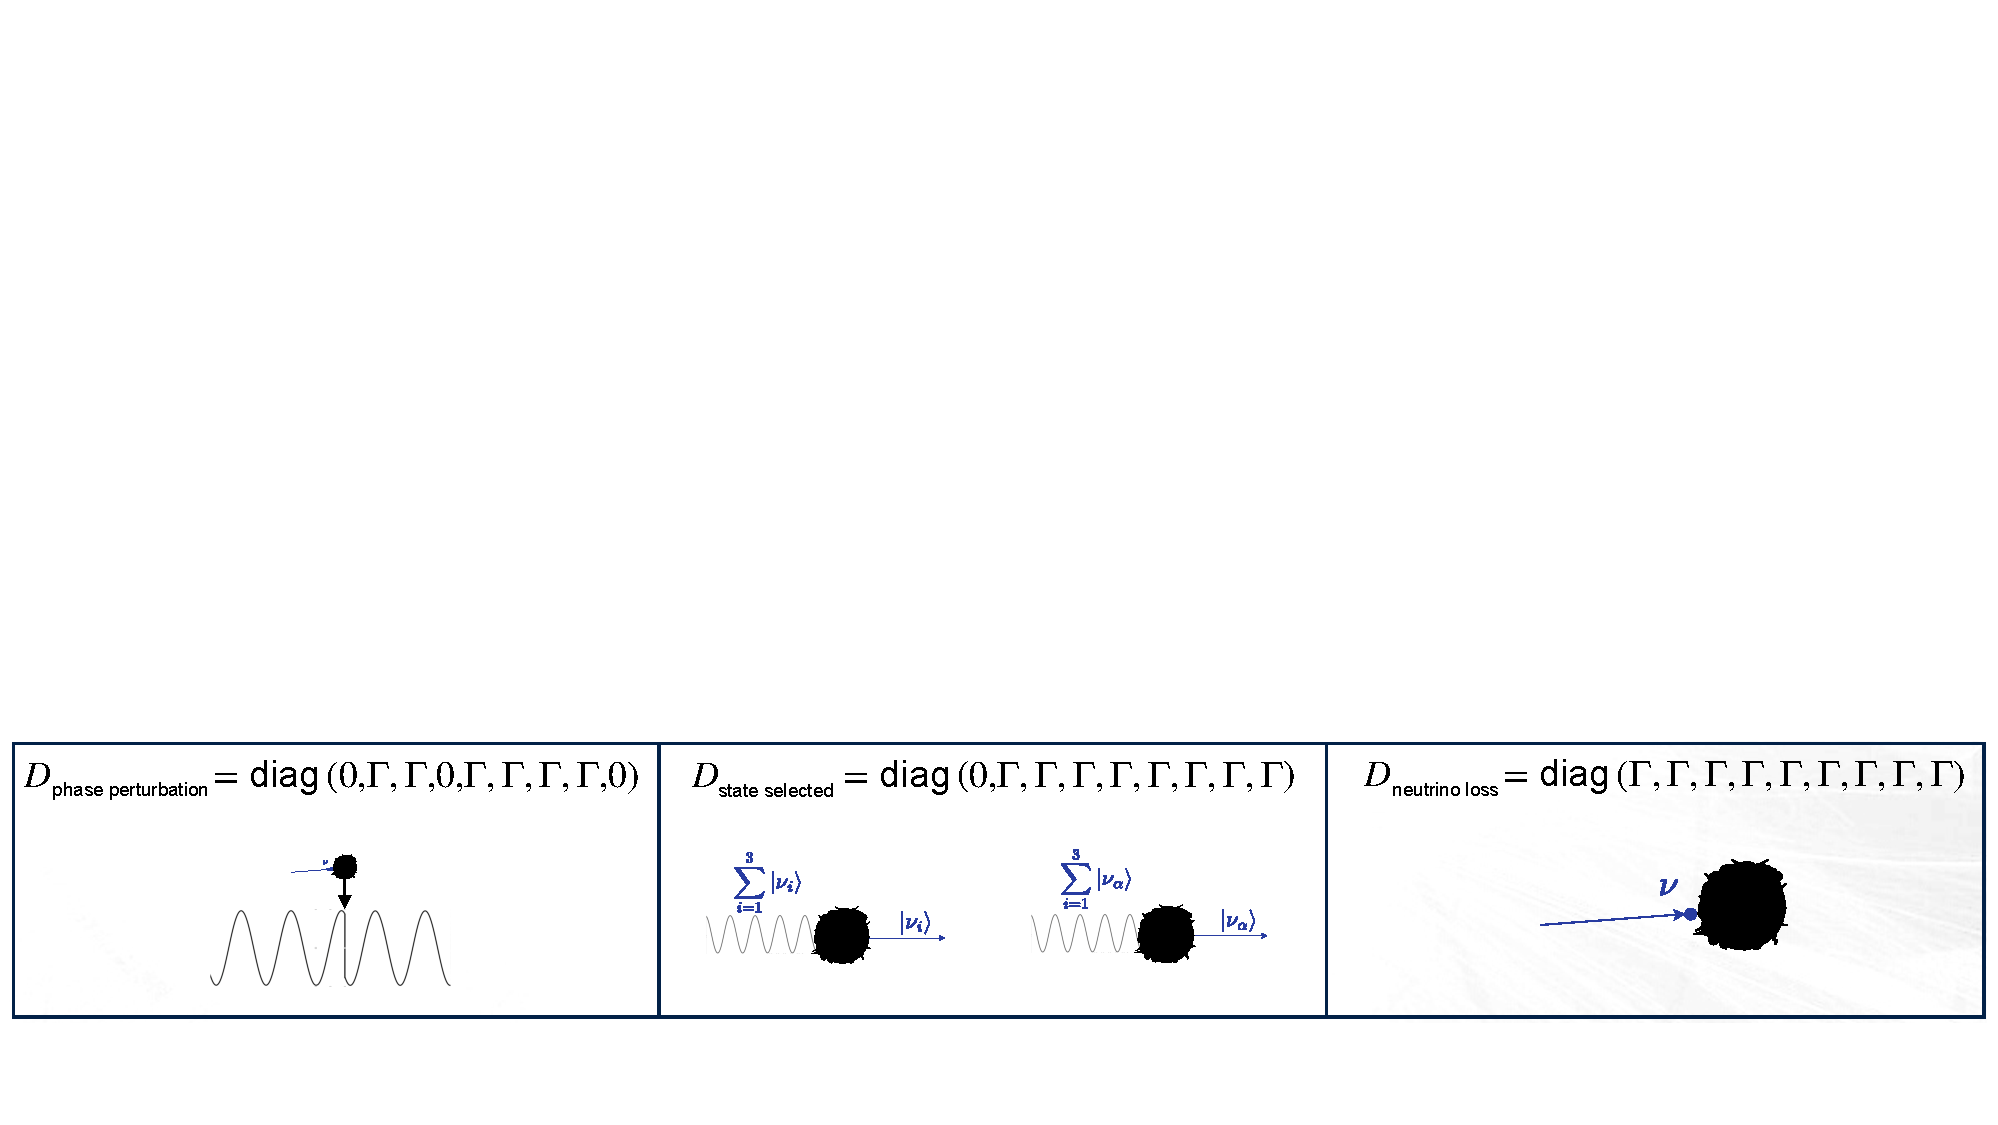
\includegraphics[width=1.\textwidth]{figures/qg_deco_models.pdf}
	\caption{Different models correspond to different decoherence matrices \cite{QD_Stutt_Jens_2020}. The neutrino-\acrshort{vbh} interaction induces left: a shift in phase, center: a neutrino flavour or mass eigenstate to be democratically selected or right: the neutrino to get lost.}
	\label{fig:qg_deco_models}
    \end{figure}
%
A power-law energy dependence of the physics producing the decoherence effects can be introduced in this parameter by \cite{QD_Stutt_Jens_2020}
\vspace{-3mm}%
\begin{align} \label{gamma-parameter}
   \Gamma(E_\nu;\Gamma(E_0), n) = \Gamma(E_0)\left( \frac{E_\nu}{E_0} \right)^n 
\end{align}
%
and is characterised by the two free parameters $\Gamma(E_0)$ and $n$. In \cref{gamma-parameter}, the reference or pivot energy scale $E_0$ [GeV] is a non-physical parameter as it is not modifying the physics when being varied, but setting the magnitude of the decoherence strength parameter $\Gamma(E_0)$. The energy scale $n$ allows one to consider different phenomenological models dependent on the choice of $n$ (see \cref{tab:energy_scale_models}):
%
\begin{table}[hbt]
    \centering
    \caption[]{Phenomenological Models according to the energy dependence of the decoherence strength $\Gamma$ set by the choice of the energy scale $n$.}
    \label{tab:energy_scale_models}
    \resizebox{\textwidth}{!}{%
        \begin{tabular}{|l|c|c|}
            \hline
             & Model & Reference \\ \hline \hline
            $n \leq -10$ & Could explain Gallium anomaly without sterile neutrinos? & \cite{Farzan:2023fqa} \\ \hline
            $n = -4$ & Decoherence due to wave-packet separation & \cite{deGouvea:2020hfl,deGouvea:2021uvg} \\ \hline
            $n = -2$ & Decoherence induced by lightcone fluctuations & \cite{Stuttard:2021uyw} \\ \hline
            $n=-1$: & Lorentz-invariant; also similar to invisible neutrino decay & \cite{Lisi:2000zt}, \cite{QD_Stutt_Jens_2020} \\ \hline
            $n=0$ & Energy-independent  & \\ \hline
            $n=+1$ & Cross-section like energy dependence or violation of quantum mechanics & \cite{Liu:1997km} \\ \hline
            $n=+2$ & Quantum Gravity motivated (high energy dependence) & \\ \hline
        \end{tabular}
    }
\end{table}
%
\iffalse
%
\begin{itemize}
    \item $n \leq -10$: Could explain Gallium anomaly without sterile neutrinos? \cite{Farzan:2023fqa}
    \item $n = -4$: Decoherence due to wave-packet separation \cite{deGouvea:2020hfl,deGouvea:2021uvg}
    \item $n = -2$: Decoherence induced by lightcone fluctuations \cite{Stuttard:2021uyw}
    \item $n=-1$: Lorentz-invariant \cite{Lisi:2000zt}; also similar to invisible neutrino decay \cite{QD_Stutt_Jens_2020}
    \item $n=0$: energy-independent 
    \item $n=+1$: Cross-section like energy dependence or see \cite{Liu:1997km} on effect of violation of quantum mechanics on neutrino oscillation
    \item $n=+2$: quantum-gravity motivated (high energy dependence)
\end{itemize}
%
\fi

The oscillation probabilities calculated from the models illustrated in \cref{fig:qg_deco_models} are shown in \cref{fig:deimos_plots} for the case where $n=2$, $\Gamma = 9.48 \times 10^{-18}$ GeV and $E_0 = 1$ GeV. For the DUNE baseline of $1300$ km, the oscillation probabilities predicted by various quantum decoherence models differ significantly from the standard $3$$\times$$3$-\acrshort{pmns} neutrino oscillation probability. Considering the T$2$K baseline of $295$ km, these differences show up in the extrema and the high energy region of the oscillation probability.
%
\begin{figure}[hbt]
	\begin{minipage}[b]{.52\textwidth}
	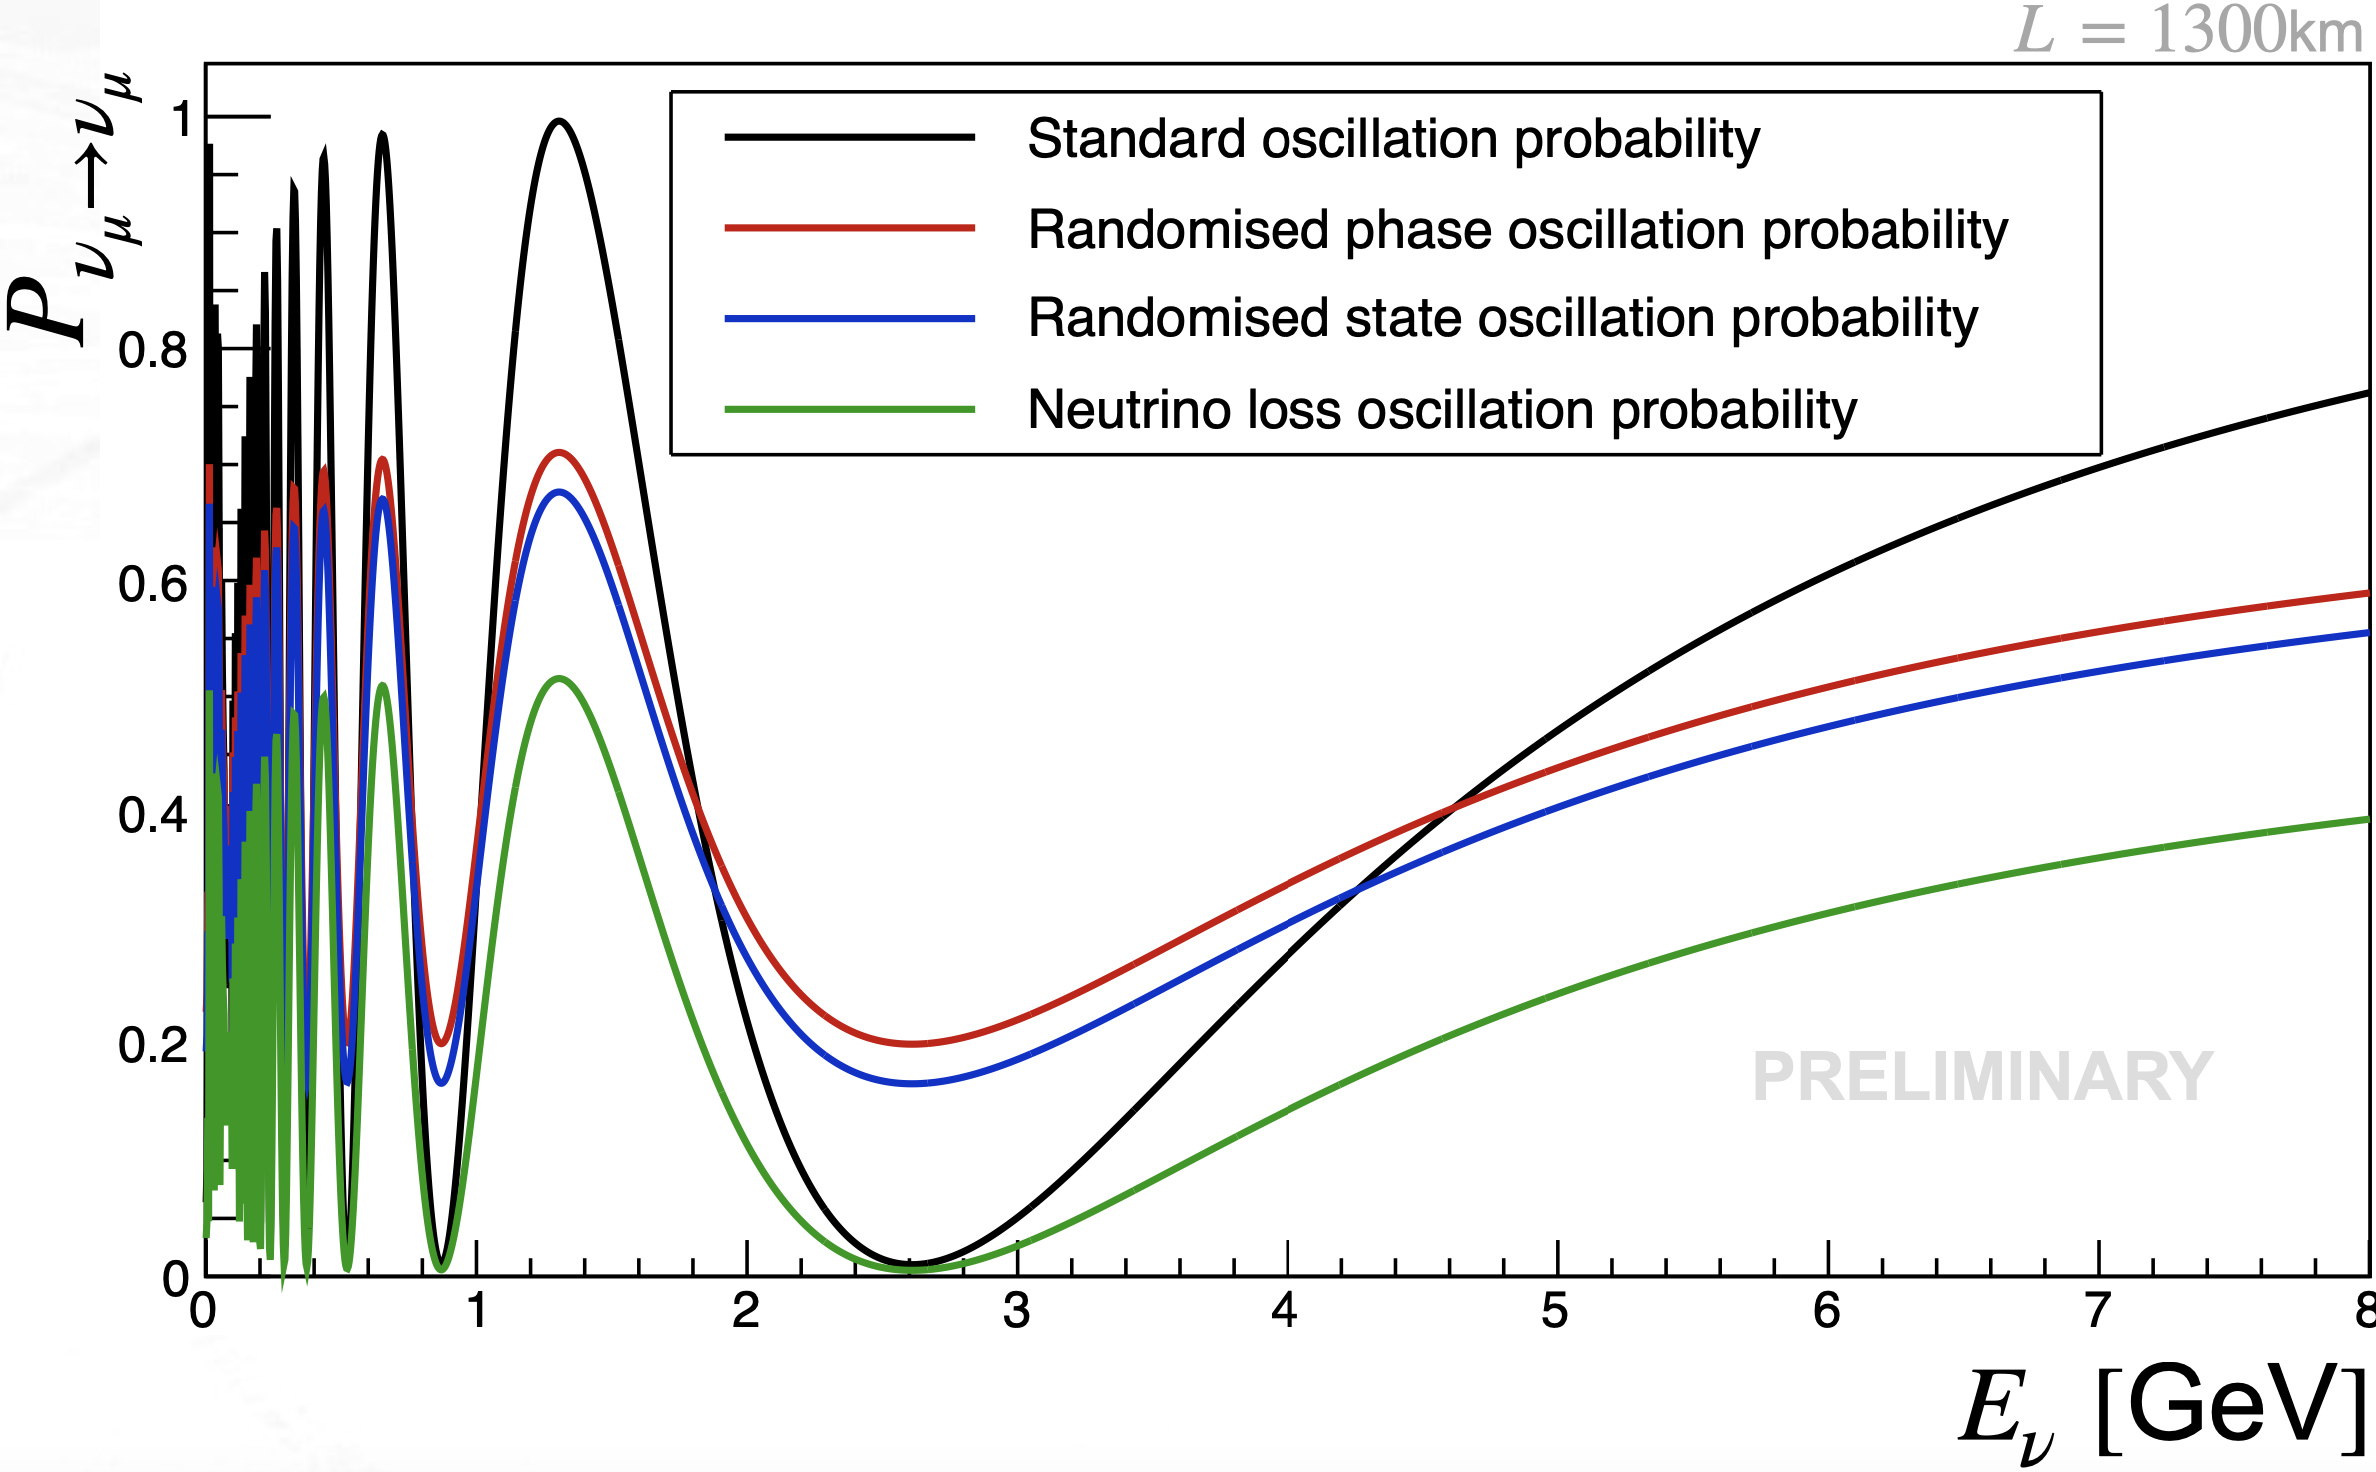
\includegraphics[width=\textwidth]{figures/deimos_probs_dune.png}
	\end{minipage}
	\begin{minipage}[b]{.485\textwidth}
	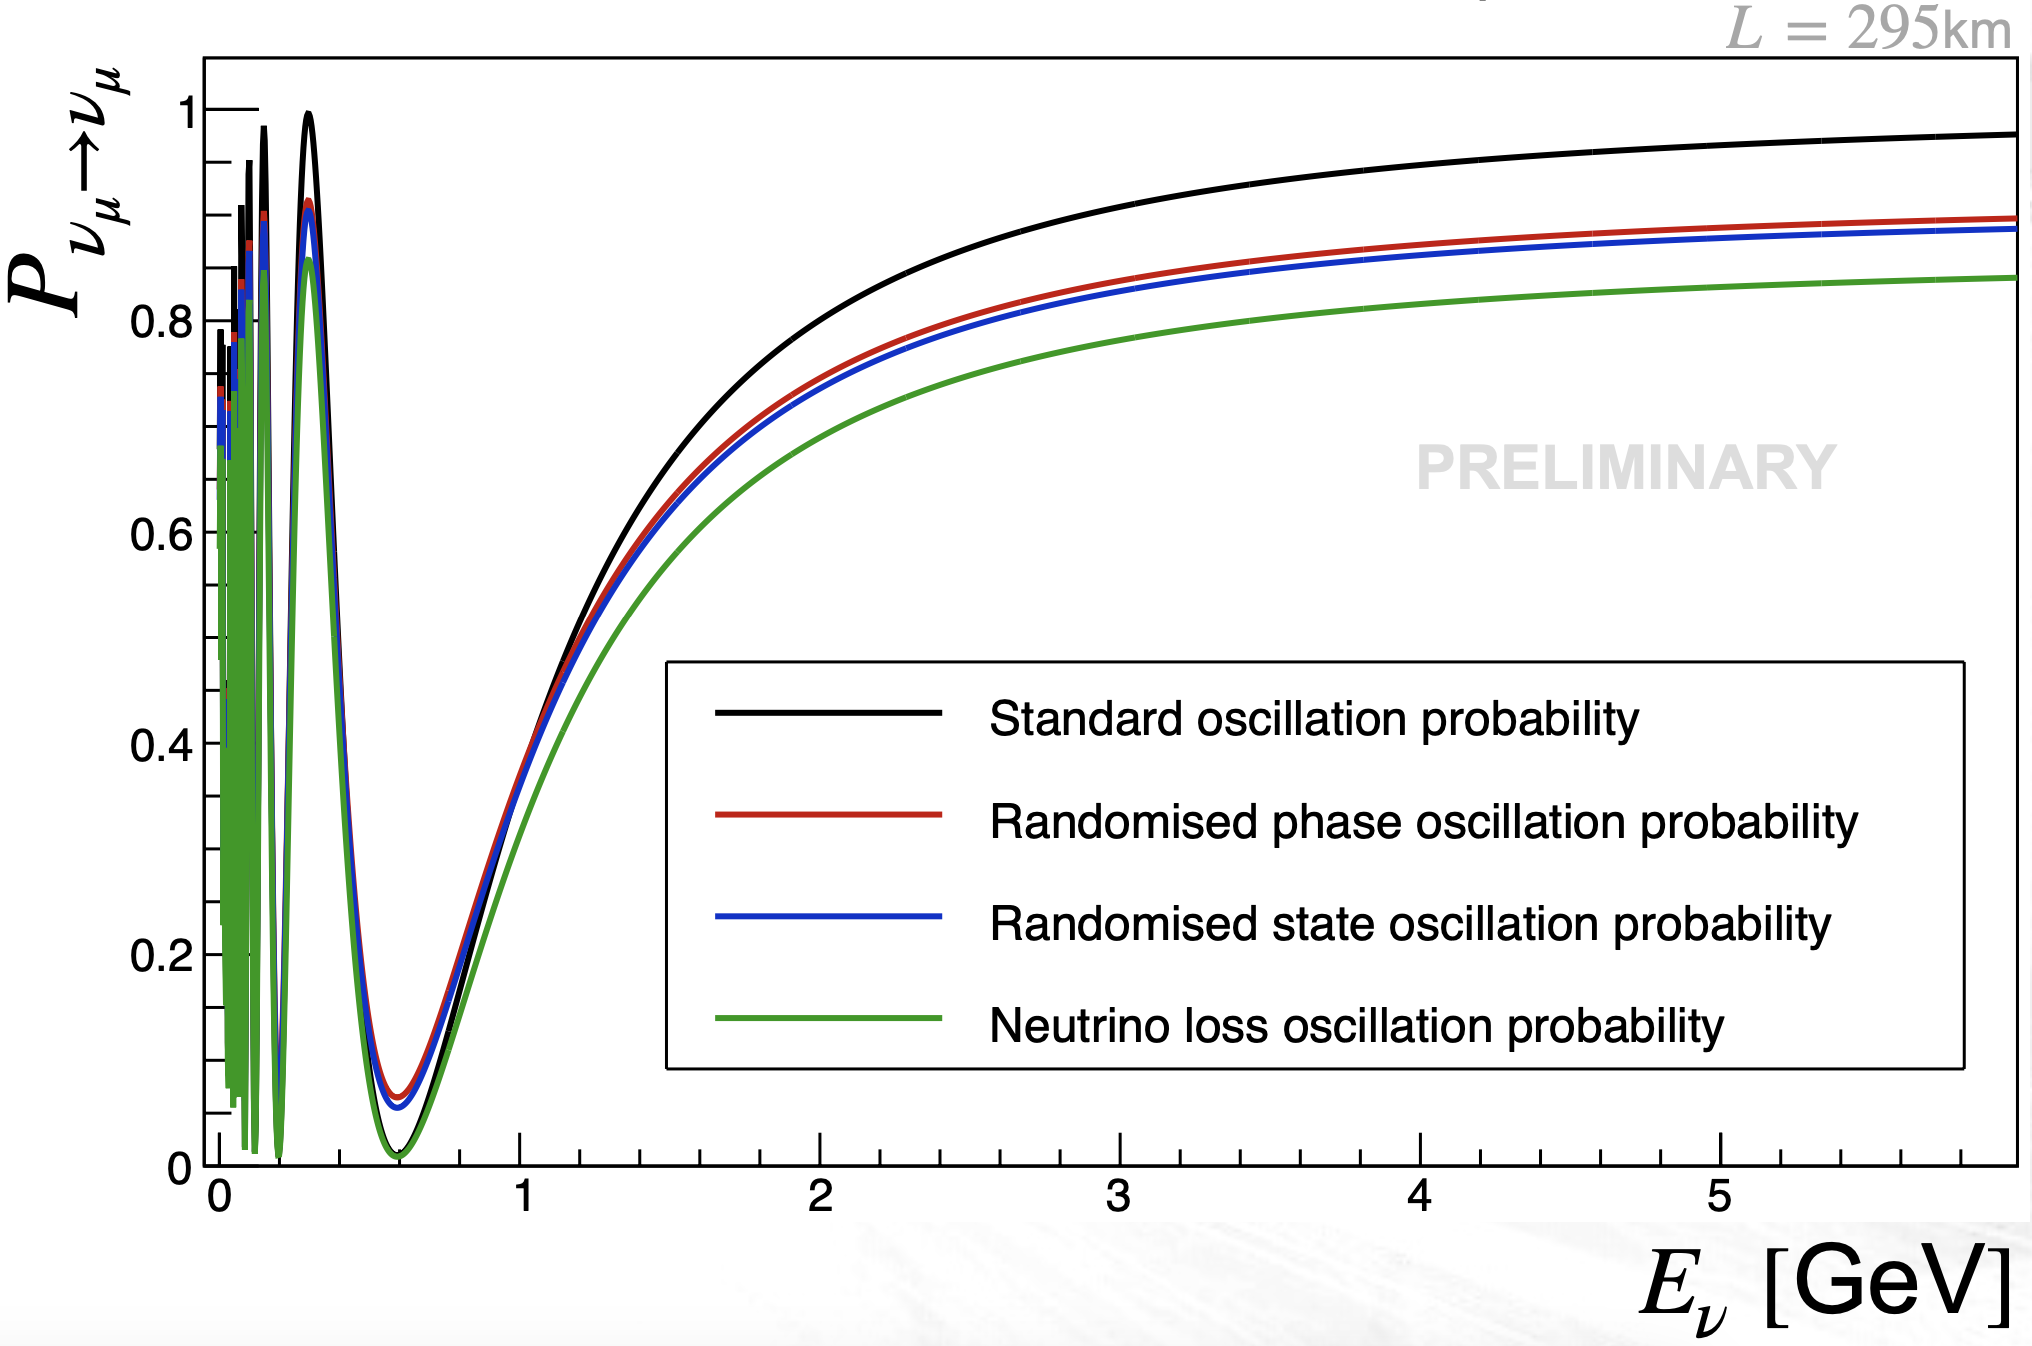
\includegraphics[width=\textwidth]{figures/deimos_probs_t2k.png}
	\end{minipage}
	\caption{The \acrshort{sm} (black), phase-perturbed (red), state-selected (blue) and neutrino loss (green) neutrino oscillation probabilities. Left: DUNE. Right: T$2$K. Plots produced with the \href{https://github.com/ts4051/deimos/tree/main}{deimos code}\cite{QD_Stutt_Jens_2020}.}
	\label{fig:deimos_plots}
\end{figure}
%
This initial study was to understand the raw ability of \acrshort{dune} and \acrshort{t2k} to observe quantum decoherence effects. It was then decided to implement quantum decoherence in the \acrshort{mach3} framework in order to investigate it in the official neutrino oscillation analyses in \acrshort{dune} and \acrshort{t2k}. 